\subsection{亏格二}%
\label{sub:Genus two}

这里讨论的亏格二镜像公式来自 Guo--Janda--Ruan~\cite{GJRgenus2}。

我们现在将在亏格二的情形下同时实现这两条路线。几何路线使用 \(t\)-扭稳定商理论，应用虚拟局部化得到五个贡献，然后应用稳定商越墙来落到五次格罗莫夫–威滕理论。形式路线使用半单 \(\lambda\)-扭理论和 \(R\)-矩阵来计算一个稳定图和。这只给出形式领头部分。然后仍然必须加上有效和亚纯的其余图。

\begin{notn}
    记
    \[ \ab<\alpha_1, \ldots, \alpha_n>^{t,\mr{SQ}}_{g,n} \coloneqq \sum_{d\geq0}q^d \int_{[\Mbar_{g,n}(\P^4,d)]^{\vir}}e(R\pi_*\mc{L}^{\otimes 5}\otimes[-1])\prod_i \ev_i^*(\alpha_i), \]
    其中 \(\mc{L}\) 是万有稳定商线丛，而 \(c_1^{\C^{\times}}([-1]) = -t\)（这是我们在下面会回到的符号约定）。这是稳定商符号约定，与上面稳定映射圈中出现的 \([1]\) 并不相同。
\end{notn}

\begin{figure}[htpb]
    \centering
    \begin{tikzpicture}[scale=0.95,transform shape]
        \draw[gray] (-0.9,0) -- (11.2,0);
        \draw[gray] (-0.9,2.2) -- (11.2,2.2);
        \node[anchor=east,gray] at (-0.9,0) {$0$};
        \node[anchor=east,gray] at (-0.9,2.2) {$\infty$};
        \node[ellipse,draw,thick,minimum width=1.5cm,minimum height=0.75cm] (a) at (0,0) {$\Sigma_2(d)$};
        \node at (0,-1) {$\Gamma^2$};
        \node[ellipse,draw,thick,minimum width=1.5cm,minimum height=0.75cm] (b0) at (2.7,0) {$\Sigma_1(d)$};
        \node[ellipse,draw,thick,minimum width=1.5cm,minimum height=0.75cm] (b1) at (2.7,2.2) {$\Sigma_1(0)$};
        \draw[thick] (b0) -- (b1);
        \node at (2.7,-1) {$\Gamma^1$};
        \node[ellipse,draw,thick,minimum width=1.5cm,minimum height=0.75cm] (c0) at (5.6,0) {$\Sigma_0(d)$};
        \node[ellipse,draw,thick,minimum width=1.5cm,minimum height=0.75cm] (c1) at (4.9,2.2) {$\Sigma_1(0)$};
        \node[ellipse,draw,thick,minimum width=1.5cm,minimum height=0.75cm] (c2) at (6.6,2.2) {$\Sigma_1(0)$};
        \draw[thick] (c0) -- (c1);
        \draw[thick] (c0) -- (c2);
        \node at (5.6,-1) {$\Gamma_b^0$};
        \node[ellipse,draw,thick,minimum width=1.5cm,minimum height=0.75cm] (d0) at (9.6,0) {$\Sigma_0(d)$};
        \node[ellipse,draw,thick,minimum width=1.5cm,minimum height=0.75cm] (d1) at (9.6,2.2) {$\Sigma_1(0)$};
        \draw[thick] (d0) to[bend left=25] (d1);
        \draw[thick] (d0) to[bend right=25] (d1);
        \node at (9.6,-1) {$\Gamma_a^0$};
    \end{tikzpicture}
    \caption{亏格二中的四个非常值局部化图，每个顶点都画成其黎曼面分支。}%
    \label{fig:g2loc}
\end{figure}

这四个非常值图绘于~\Cref{fig:g2loc}，它们的贡献为
\begin{align*}
    \Cont_{\Gamma^2} &= \ab<>^{t,\mr{SQ}}_{2,0}, \\
    \Cont_{\Gamma^1} &= -\ab< \frac{-\frac{5}{2}H^3 + \frac{5}{24}H^4t^{-1}}{(t-5H)(t-5H-\psi)}>^{t,\mr{SQ}}_{1,1}, \\
    \Cont_{\Gamma_b^0} &= \ab< \frac{-\frac{5}{2}H^3+\frac{5}{24}H^4t^{-1}}{(t-5H)(t-5H-\psi_1)}, \frac{-\frac{5}{2}H^3+\frac{5}{24}H^4t^{-1}}{(t-5H)(t-5H-\psi_2)}>^{t,\mr{SQ}}_{0,2},
\end{align*}
而对于双边的图，记 \(H_1 = H \otimes 1\) 和 \(H_2 = 1 \otimes H\)，
\[ \Cont_{\Gamma_a^0} = \ab< \frac{\frac{5}{3}(H^3\otimes H^4 + H^4 \otimes H^3)t^{-1} + \frac{65}{24}H^4 \otimes H^4 t^{-2}}{(t-5H_1)(t-5H_1-\psi_1)(t-5H_2)(t-5H_2-\psi_2)}>^{t,\mr{SQ}}_{0,2}. \]
注意这些关联函数位于 \(\P^4\) 上，因此 \(H^4\) 出现且非零。

来自零次图还有第五个贡献，它是一个常数
\[ -2c_{2,0} = -\frac{5}{144}, \qquad c_{2,0} = -\frac{1}{2}N_{2,0} = \frac{5}{288}, \]
把五个贡献相加，我们得到局部化恒等式
\[ F_2^{\mr{SQ}}(q) = \Cont_{\Gamma^2} + \Cont_{\Gamma^1} + \frac{1}{2}\Cont_{\Gamma_a^0} + \frac{1}{2}\Cont_{\Gamma_b^0} - 2c_{2,0}, \]
其中两个因子 \(\frac{1}{2}\) 是 \(\Gamma_a^0\) 和 \(\Gamma_b^0\) 的自同构。

设 \(Q = qe^{\tau(q)}\) 和 \(L = (1-5^5q)^{-1/5}\)，其中 \(\tau(q) = I_1(q)/I_0(q) - \log q\) 是通常的镜像平移。我们现在应用稳定商越墙来得到精确恒等式
\[ F_2^{\mr{GW}}(Q) = I_0(q)^2 F_2^{\mr{SQ}}(q). \]
引入 \(D_u = L^{-1}q\odv{}{q}\) 和生成元
\[ \mc{X}_k = D_u^k \log \frac{I_0}{L}, \qquad \mc{Y}_k = D_u^k \log \frac{I_0I_{1,1}}{L^2}, \qquad I_{1,1} = 1 + q \odv{\tau}{q}, \quad D_u L = \frac{1}{5}(L^5-1), \]
各个扭图的贡献还会涉及额外的生成元。对我们而言重要的一点是，它们在上面的线性组合中会相消，并恰好留下有限生成的变量。记 \(X = \mc{X}_1\) 和 \(Y_1 = \mc{Y}_1\)，我们得到
\begin{align*}
    F^{\mr{GW}}_2(Q) = \frac{I_0^2}{L^2}\Big(&\frac{70}{9}\mc{X}_3 + \frac{575}{18}X\mc{X}_2 + \frac{557}{72}X^3 + \frac{5}{6}Y_1\mc{X}_2 \\
    &- \frac{629}{72}Y_1X^2 - \frac{23}{24}Y_1^2 X - \frac{1}{24}Y_1^3 \\
    &+ \frac{125}{36}\mc{X}_2 L^4 - \frac{5}{24}X^2L^4 - \frac{35}{9}Y_1XL^4 - \frac{5}{24}Y_1^2L^4 \\
    &- \frac{1441}{300}XL^3 - \frac{41}{300}Y_1L^3 + \frac{31459}{7200}XL^8 + \frac{2141}{7200}Y_1L^8 \\
    &+ \frac{29621}{12000}L^{12} - \frac{116369}{36000}L^7 + \frac{547}{750}L^2\Big).
\end{align*}
如果在大半径处展开，那么我们得到
\[ F_2^{\mr{GW}}(Q) = -\frac{5}{144} + \frac{575}{48}Q + \frac{5125}{2}Q^2 + \frac{7930375}{6}Q^3 + O(Q^4), \]
这些系数是格罗莫夫–威滕不变量 \(N_{2,d}\)，而不是~\Cref{tab:quinticbps} 的 BPS 整数。

我们现在转向形式路线。\(\Omega^{\lambda}_{2,0}\) 的 Givental-Teleman 公式是亏格二无脚七种稳定图上的一个和，这些图绘于~\Cref{fig:g2stable}。只需要到 \(z^3\) 的 \(R^{-1}(z)\)，而这些平移把七种拓扑展开成 \(17\) 个带装饰的层。

\begin{figure}[htpb]
    \centering
    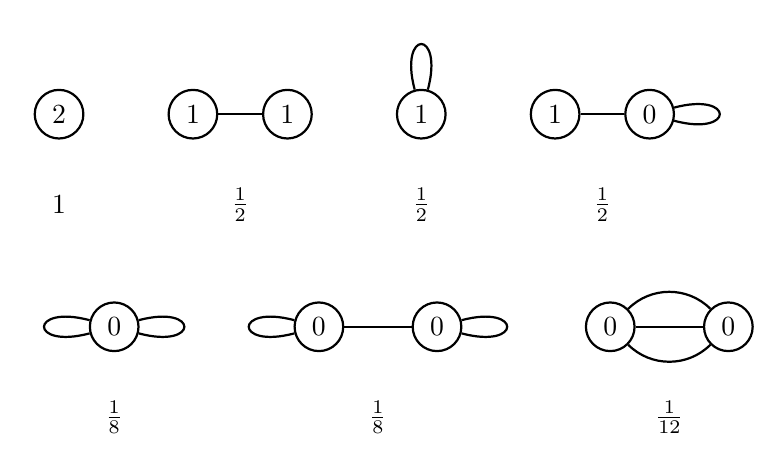
\begin{tikzpicture}[scale=1,transform shape,every loop/.style={min distance=8mm,looseness=10}]
        \node[circle,draw=black,thick] (a) at (0,0) {$2$};
        \node at (0,-1.15) {$1$};

        \node[circle,draw=black,thick] (b1) at (1.7,0) {$1$};
        \node[circle,draw=black,thick] (b2) at (2.9,0) {$1$};
        \draw[thick] (b1) -- (b2);
        \node at (2.3,-1.15) {$\frac{1}{2}$};

        \node[circle,draw=black,thick] (c) at (4.6,0) {$1$};
        \draw[thick] (c) edge[loop above] (c);
        \node at (4.6,-1.15) {$\frac{1}{2}$};

        \node[circle,draw=black,thick] (d1) at (6.3,0) {$1$};
        \node[circle,draw=black,thick] (d2) at (7.5,0) {$0$};
        \draw[thick] (d1) -- (d2);
        \draw[thick] (d2) edge[loop right] (d2);
        \node at (6.9,-1.15) {$\frac{1}{2}$};

        \node[circle,draw=black,thick] (e) at (0.7,-2.7) {$0$};
        \draw[thick] (e) edge[loop left] (e);
        \draw[thick] (e) edge[loop right] (e);
        \node at (0.7,-3.85) {$\frac{1}{8}$};

        \node[circle,draw=black,thick] (f1) at (3.3,-2.7) {$0$};
        \node[circle,draw=black,thick] (f2) at (4.8,-2.7) {$0$};
        \draw[thick] (f1) -- (f2);
        \draw[thick] (f1) edge[loop left] (f1);
        \draw[thick] (f2) edge[loop right] (f2);
        \node at (4.05,-3.85) {$\frac{1}{8}$};

        \node[circle,draw=black,thick] (g1) at (7.0,-2.7) {$0$};
        \node[circle,draw=black,thick] (g2) at (8.5,-2.7) {$0$};
        \draw[thick] (g1) -- (g2);
        \draw[thick] (g1) to[bend left=45] (g2);
        \draw[thick] (g1) to[bend right=45] (g2);
        \node at (7.75,-3.85) {$\frac{1}{12}$};
    \end{tikzpicture}
    \caption{亏格二无脚的七种稳定图，以顶点的亏格标记，并以 \(\frac{1}{\ab|\Aut\Gamma|}\) 加权。在幻灯片上，每个顶点都画成其黎曼面分支。}%
    \label{fig:g2stable}
\end{figure}

\begin{rmk}
    这些是稳定曲线的对偶图，不是~\Cref{fig:tropgraphs} 的图，后者是把热带分解公式应用于对数 GLSM 的约化理论所得到的刚性热带型。这两组拓扑在此恰好重合，但顶点在其中的含义不同。这里它是一个承载拓扑场论张量的定义域曲线的分支。那里它是一个二分热带曲线的层级，承载对数或 \(\infty\)-顶点模问题。
\end{rmk}

对于形式路线，我们通过
\[ P_2^{\lambda} \coloneqq \frac{Y}{I_0^2}F_2^{\lambda}, \qquad Y = L^5. \]
内蕴地定义归一化势。完全的图和位于 \(\Q[L,\mc{X}_1,\mc{X}_2,\mc{X}_3,\mc{Y}_1]\) 中，等于
\begin{align*}
    P_2^{\lambda} ={}& -\frac{1}{128}L^{12} - \frac{23}{960}L^8\mc{X}_1 - \frac{9}{640}L^8\mc{Y}_1 + \frac{109}{16000}L^7 \\
    &- \frac{3}{80}L^4\mc{X}_1^2 - \frac{19}{320}L^4\mc{X}_1\mc{Y}_1 - \frac{3}{80}L^4\mc{Y}_1^2 - \frac{1}{64}L^4\mc{X}_2 \\
    &+ \frac{19}{1920}L^3\mc{X}_1 - \frac{47}{48000}L^2 \\
    &- \frac{67}{1152}\mc{X}_1^3 - \frac{101}{1152}\mc{X}_1^2\mc{Y}_1 - \frac{5}{48}\mc{X}_1\mc{Y}_1^2 - \frac{1}{24}\mc{Y}_1^3 \\
    &- \frac{25}{288}\mc{X}_1\mc{X}_2 - \frac{1}{48}\mc{X}_2\mc{Y}_1 - \frac{19}{1152}\mc{X}_3.
\end{align*}
为清楚起见，这是精确的形式 \(\lambda\)-扭答案，而不是 \(F_2^{\mr{GW}}\)。还要注意 \(Y = L^5\) 是判别式生成元，而 \(\mc{Y}_1\) 是对数导数生成元。

\subsection{有限生成与扩张族}%
\label{sub:Finite generation and the extended family}

回忆上面有限生成的环 \(\mc{R} = \Q[A,B_1,B_2,B_3,Y]\)，我们将用
\[ \deg A = \deg B_1 = 1, \qquad \deg B_2 = 2, \qquad \deg B_3 = 3, \qquad \deg Y = 0. \]
来分次。对于和之前一样的 \(\phi_k = I_{1,1}\cdots I_{k,k}H^k\)，设
\[ \wt{\Omega}^{\lambda}_{g,n} \coloneqq 5^{g-1}\ab(\frac{Y}{I_0^2})^{g-1}\Omega^{\lambda,\tau}_{g,n}. \]

\begin{thm}[分次有限生成 {\cite{GJRstructure}}]%
\label{thm:graded finite generation}
    我们有
    \[ \wt{\Omega}^{\lambda}_{g,n}(\phi_{a_1}, \ldots, \phi_{a_n}) \in \bigoplus_{k \geq 0}\lambda^{5k}H^{2(3g-3+\sum_i a_i - 5k)}(\Mbar_{g,n},\Q)\otimes \mc{R}_{3g-3+\sum_i a_i}. \]
    因此，在组装二分其余图之后，扩张族的非等变分量满足
    \[ P^{\mbf{C}}_{g,n} = 5^{1-g}\int_{\Mbar_{g,n}}\wt{\Omega}^{\mbf{C}}_{g,n}(\phi_1^{\otimes n}) = \ab( \frac{Y}{I_0^2})^{g-1}\int_{\Mbar_{g,n}}\Omega^{\mbf{C}}_{g,n}(\phi_1^{\otimes n}) \in \mc{R}_{3g-3+n}. \]
\end{thm}

特别地，在每一固定 \((g,n)\) 处只能出现有限多个分次单项式，并且只有阶数不超过 \(3g-3+n\) 的 \(R\)-矩阵能作出贡献。

我们用二分图和
\[ \Omega^{\mbf{C},\lambda}_{g,n} = \sum_{\Gamma \text{ bipartite}} \frac{1}{\ab|\Aut\Gamma|}\prod_{v\in V_{\infty}(\Gamma)} C^{\infty}_{g_v,\mu_v}(\mbf{C};\vec{a}_v) \prod_{v \in V_0(\Gamma)}C^{\lambda}_{g_v,\vec{\delta}_v}(\vec{a}_v)\prod_{e \in E(\Gamma)}V_e, \]
来组织扩张理论，其中 \(C^{\infty}\) 是有效或亚纯顶点因子，\(C^{\lambda}\) 是形式零顶点关联函数，\(\mu_v\) 和 \(\vec{\delta}_v\) 记录各关联次数，而 \(V_e\) 是边因子。极限 \(\lambda \to 0\) 只在完成图和之后才取。令 \(\mbf{C}=0\) 就留下形式 \(\lambda\)-扭领头扇区。令 \(\mbf{C}=\mbf{C}^{\mr{eff}}\) 并令 \(\lambda\to0\) 就恢复五次格罗莫夫–威滕理论。对万有边求导会把它切开并产生全纯反常方程，同时保持有效顶点不受影响。

为推导全纯反常方程，记 \(P^{\mbf{C}}_g \coloneqq P^{\mbf{C}}_{g,0}\) 并引入
\[ \mc{U} = B_1, \qquad \mc{V} = A + 2B_1, \qquad \mc{V}_2 = D\mc{U} + \mc{U}^2 - \mc{U}\mc{V}, \qquad \mc{V}_3 = (D+\mc{V})\mc{V}_2, \]
连同两个非全纯方向
\[ \partial_1 = \partial_{\mc{U}}, \qquad \partial_0 = \partial_{\mc{V}} - \mc{U}\partial_{\mc{V}_2} - \mc{U}^2\partial_{\mc{V}_3}. \]

\begin{thm}[扩张族的全纯反常方程 {\cite{GJRstructure}}]
    我们有
    \[ -\partial_0 P^{\mbf{C}}_g = \frac{1}{2}P^{\mbf{C}}_{g-1,2} + \frac{1}{2}\sum_{\substack{g_1+g_2=g\\g_1,g_2\geq1}}P^{\mbf{C}}_{g_1,1}P^{\mbf{C}}_{g_2,1}, \qquad -\partial_1 P^{\mbf{C}}_g = 0. \]
\end{thm}

我们通过~\Cref{sub:The holomorphic anomaly equation} 的切割论证来证明这一点，该论证之所以可行，是因为 \(R\)-矩阵传播子的导数正好是
\[ 5\mc{B}_{\partial_0} = \bar{\phi}_1 \otimes \bar{\phi}_1, \qquad 5\mc{B}_{\partial_1} = \bar{\phi}_0\otimes\bar{\phi}_2 + \bar{\phi}_2\otimes\bar{\phi}_0. \]
\(R^{-1}\) 和每条边的导数都留在同一个分次环内，所以切割一条被求导的边会闭合到 \(\mc{R}\) 中亏格更低的关联函数上。如果令 \(\mbf{C}=0\)，那么我们就得到形式 \(\lambda\)-扭理论的同样方程。

\subsection{边界条件}%
\label{sub:Boundary conditions}

我们将使用两个来源的全纯歧义条件。

首先，我们使用在轨形点或 Landau-Ginzburg 点 \(q = \infty\) 处，等价地在 \(L \to 0\) 处的正则性。对于形式势或组装后的扩张势 \(F_g^{\star}\)，设
\[ \mc{P}_g^{\mr{orb},\star} \coloneqq \ab(\frac{L}{I_0})^{2g-2}F_g^{\star} = \Phi_g^{\star}(\mc{X}_1,\mc{X}_2,\mc{X}_3,\mc{Y}_1,L^{-1},L^5). \]
\Cref{thm:graded finite generation} 给出了 \(L\) 的可能 Laurent 幂次的界，而形式 LG/CY 等同断言：在解析延拓并等同归一化的 CY 基和 LG 基之后，同一个形式 \(R\)-矩阵多项式描述两个相。因此
\[ \lim_{L\to0}\Phi_g^{\star}(\mc{X}_1,\mc{X}_2,\mc{X}_3,\mc{Y}_1,L^{-1},L^5) \text{ exists}, \]
而对于 \(f_g(Y) = \sum_{i=0}^{3g-3}a_{i,g}Y^i\) 且 \(Y = L^5\)，五次界是
\[ a_{i,g} = 0 \qquad \text{for } i \leq \ceil*{\frac{3(g-1)}{5}}. \]
注意这是关于组装后的归一化图贡献的陈述，而不是关于单个裸亚纯或橡胶顶点关联函数的陈述。

其次，我们研究锥形点。设
\[ q = 5^{-5}(1+t_c)^{-1}, \qquad T_c = \frac{I_1^{\mr{co}}(t_c)}{I_0^{\mr{co}}(t_c)}, \]
其中 \(I_0^{\mr{co}}, I_1^{\mr{co}}\) 构成一对局部锥形点的周期，其归一化使得消没的平坦坐标在锥形点处满足 \(T_c = 0\)。给定有限生成数据中的一个有理表达式 \(f\)，我们通过把一切生成元的 Laurent 展开代成 \(T_c\) 的级数来得到它的锥形点值 \(f^{\mr{co}}\)。\Cref{thm:graded finite generation} 给出极点界
\[ F_g^{\mbf{C},\mr{co}} = O\ab(T_c^{-(2g-2)}), \]
但我们所需要的是更强的 \textit{间隙} 条件
\[ F_g^{\mr{co}} = \frac{c_g}{T_c^{2g-2}} + O(1), \]
即每个中间负幂 \(T_c^{-(2g-3)}, \ldots, T_c^{-1}\) 都消没。这是 \(2g-2\) 个条件，且并不由有限生成推出。

\begin{conj}[形式锥形点间隙]%
\label{conj:formal conifold gap}
    形式 \(\lambda\)-扭势具有万有领头项
    \[ F_g^{\lambda,\mr{co}} = \frac{(-1)^{g-1}B_{2g}}{2g(2g-2)T_c^{2g-2}} + O(1), \]
    其中 \(B_{2g}\) 是伯努利数。
\end{conj}

\begin{exm}
    在亏格二中，计算出的展开开头为
    \[ F_2^{\lambda,\mr{co}} = \frac{1}{240T_c^2} + \frac{31}{6000} - \frac{7169}{3600000}T_c + \frac{22951}{45000000}T_c^2 + O(T_c^3). \]
    这是亏格二的间隙，而不仅仅是极点阶数的界。
\end{exm}

我们还必须考虑带有有理后代插入的形式关联函数，它们出现在其余图中，即
\[ C^{\lambda}_{g,\vec{\delta}}(\vec{a}) \coloneqq \ab< \frac{H^{3-a_1}}{-5H\ab(-\frac{5H}{\delta_1}-\psi_1)}, \ldots, \frac{H^{3-a_n}}{-5H\ab(-\frac{5H}{\delta_n}-\psi_n)}>^{\lambda}_{g,n} \]
其中 \(\delta_i \geq 1\)，\(a_i \in \ab\{0,1,2,3,4\}\)。

\begin{conj}[带特殊插入的正则性]%
\label{conj:special correlator regularity}
    我们有 \(\ab(C^{\lambda}_{g,\vec{\delta}}(\vec{a}))^{\mr{co}} = O(1)\)。
\end{conj}

对于固定的 \(\vec{a}\) 和 \(\vec{\delta}\)，\(\psi\)-展开中的单项可能具有极点。注意该断言涉及完全的有理后代插入，其负幂在取剩余图对 \(\vec{a}\) 的和之前就已经相消。这是关于这些特定形式关联函数的陈述，而不是关于每个未组装的亚纯关联函数的陈述。

我们可以利用~\Cref{conj:formal conifold gap,conj:special correlator regularity} 把间隙转移到五次格罗莫夫–威滕理论。一个其余图贡献具有形状
\[ \sum_{\vec{a}} \prod_{v \in V_{\infty}(\Gamma)}I_0^{2g_v-2+\ell(\mu_v)}C^{\infty}_{g_v,\mu_v}(\vec{a}_v)\prod_{v\in V_0(\Gamma)}C^{\lambda}_{g_v,\vec{\delta}_v}(\vec{a}_v), \]
而 \(C^{\infty}\) 因子是 \(q\) 的有限多项式，因此它们在锥形点处正则。于是形式领头间隙连同特殊关联函数的正则性一起蕴含扩张族的间隙，从而蕴含五次的间隙。

\begin{rmk}
    \Cref{conj:formal conifold gap,conj:special correlator regularity} 一般仍是未决的，但 Guo-Janda-Ruan 已经把五次的情形验证到 \(g \leq 5\)。扩张族的极点界是一个定理，而间隙由这两个猜想推出，并通过显式计算对 \(g \leq 5\) 得到证明。在这些讲座之时，五次格罗莫夫–威滕理论的全亏格间隙因此以它们为条件，而对 \(g \leq 5\) 是无条件的。\footnote{随后，Chang--Guo--You--Zhang 在~\cite{CGYZ2026} 中宣布了五次格罗莫夫–威滕理论锥形点间隙的全亏格证明。上面两个形式理论的猜想是彼此独立的陈述。}
\end{rmk}

把这一切放在一起，我们从 Picard-Fuchs 数据出发，计算 Givental \(R\)-矩阵和算子 \(S_{\tau}(z)\)。然后我们得到形式稳定图和亚纯其余图，使用全纯反常方程和有限生成，最后施加轨形点与锥形点边界条件来确定 \(F_g^{\mr{GW}}\)。
